% bib
%bibrefs
\documentclass[output=paper]{LSP/langsci} 
\author{Kristín Bjarnadóttir\affiliation{The Árni Magnússon Institute
 for Icelandic Studies, University of Iceland}
}
\title{Phrasal compounds in Modern Icelandic with reference to Icelandic word formation in general} 
\shorttitlerunninghead{Phrasal compounds in Modern Icelandic}  
\abstract{In Icelandic, as in many other languages, phrasal compounds are an interface phenomenon of the different components of grammar. The rules of syntax seem to be preserved in the phrasal component of Icelandic compounds, as they show full internal case assignment and agreement. Phrasal compounds in Icelandic can be divided into two distinct groups. The first group contains common words which are part of the core vocabulary irrespective of genre, and these are not stylistically marked in any way. Examples of these structures can be found in texts from the 13th century onwards. The second group contains more complex compounds, mainly found in informal writing, as in blogs, and in speech. These seem to be 20th century phenomena. Phrasal compounds of both types are relatively rare in Icelandic, but other types of compounding are extremely productive. Traditionally, Icelandic compounds are divided into two groups, i.e., compounds containing stems and compounds containing inflected word forms, mostly genitives, as non-heads.  Phrasal compounds in Icelandic also have genitive non-heads, raising questions on the difference between the processes in non-phrasal and phrasal compounding in Icelandic.
}

\ChapterDOI{10.5281/zenodo.885105}
\maketitle

\begin{document} 

\section{Introduction}

Compounding is extremely productive in \ili{Icelandic}, and an indication of this can be seen in the proportions of non-compounds (base words) vs. compounds in The Database of Modern \ili{Icelandic} Inflection (DMII, \citealt{Bjarnadóttir2012}), a full-form database of inflectional forms produced at The Árni Magnússon Institute for \ili{Icelandic} Studies and its forerunner, The Institute of Lexicography.\footnote{The DMII was initially conceived as a language resource for natural language processing, but was also intended for use in lexicography and linguistic research. The paradigms are accessible online as a reference tool and are used as such by the general public. Downloadable data and website: http://bin.arnastofnun.is.} The DMII contains the core vocabulary of Modern \ili{Icelandic}, with approximately 280,000 paradigms. The vocabulary is not selected by morphological criteria, apart from the self-explanatory fact that only inflected words are included.  The sources of the DMII are lexicographic data, both from traditional dictionary archives and corpora. Out of 278,764 paradigms in the DMII on Dec. 15th 2015, 32,118 entries were non-compounds, and the remaining 246,646 entries were compounds. The DMII contains both lexicalized compounds and purely productive ones, but the same rules of word formation pertain to both, i.e., they are morphologically identical. 

The DMII only contains compounds written as continuous strings, in accordance with current \ili{Icelandic} spelling conventions. These spelling conventions are a feature of Modern \ili{Icelandic} and they do not hold in older forms of the language. To give a very simple and common example, patronyms are written as a continuous string in Modern \ili{Icelandic}, e.g. \textit{Bjarnadóttir} `daughter of Bjarni’, not \textit{Bjarna dóttir} as evidenced in older texts. Residues of the older spelling are still found in some instances in Modern \ili{Icelandic}, as when the names of the sagas are written discontinuously: \textit{Njáls saga} `The Story of Burnt Njáll’. This is traditional in the names of the sagas and recommended in the current spelling rules for \ili{Icelandic}, but otherwise the continuous string is the norm. Spelling mistakes in present-day \ili{Icelandic} do, however, very often involve the splitting of compounds, and these are most commonly found in informal texts where phrasal compounds (PCs) are very often found. These problems with spelling make PCs elusive both in traditional lexicographic archives and in automatic word extraction. PCs are here taken to be compounds where the non-head contains any kind of syntactic phrase, from noun phrases and \isi{prepositional} phrases up to full finite sentences.

Discussion of PCs is largely absent from the linguistic literature on \ili{Icelandic}, and probably first mentioned in \citealt{Bjarnadóttir19962005}, citing examples not adhering to \citegen{Botha1981} No Phrase Constraint. The \ili{Icelandic} examples cited in \citealt{Bjarnadóttir19962005} are now a part of a private collection of over 200,000 \ili{Icelandic} compounds, with full analysis of structure and constituent parts. The sources for this collection are to a large extent the same as for the DMII. The following analysis of PCs is based on this collection, with approx. 200 additional PCs from other sources, such as \textit{Íslenskur orðasjóður} (Wortschatz, University of Leipzig, see \citealt{HallsteinsdóttirEtAl2007}), a corpus of texts from \ili{Icelandic} websites, which is a good source of informal language. The total number of PCs used in this study is approx. 900. The problems involved in finding the more informal PCs are described in \sectref{sec:bjarnadottir:3}, cf. \REF{ex:bjarnadottir:14}. At the present stage of technology, the data is sparse, and the full picture of PCs in \ili{Icelandic} therefore awaits a better analysis of multiword lexical items.

%References to Sections left as "\sectref{sec:bjarnadottir:3}. I could not find a source.
%References to Examples: \ref{ex:bjarnadottir:14}

In this study, PCs in Modern \ili{Icelandic} are divided into two groups, based on structure, and usage or genre. The first group (Phrasal Compounds I, PCIs) contains structures which are attested by examples from the 13th century onwards, as in the Dictionary of Old Norse Prose (ONP). These PCIs are very much a feature of Modern \ili{Icelandic}, they are not marked in any way stylistically, and they may appear in any genre. The most common structures of phrasal non-heads in this group are \isi{prepositional} phrases (\ref{ex:bjarnadottir:1a}), and \isi{genitive} noun phrases (\ref{ex:bjarnadottir:1b}), both showing full \isi{inflection} or agreement:\footnote{The compounds are aligned to the glosses, but \ili{Icelandic} spelling conventions stipulate that they are written continuously. Hyphens are shown when part of the spelling.}


\ea%1
 \label{ex:bjarnadottir:1} 
\ea \label{ex:bjarnadottir:1a} 
\gll milli ríkja samningur\\
 between.\textsc{prep} state.\textsc{n.neut.gen.pl} contract.\textsc{n.masc}\\
\glt ‘international agreement’

\ex\label{ex:bjarnadottir:1b}
\gll tveggja manna far\\
 two.\textsc{num.gen.pl} man.\textsc{n.masc.gen.pl} vehicle\\

\glt ‘a boat for two’  
\z
\z

The second group (Phrasal Compounds II, PCIIs) contains PCs that are found in certain informal genres, i.e., in blogs, social media, and speech, etc. All the examples are recent, they are often considered a little strange, and the question “Is this really a word?” is sometimes heard in connection with them. The structure of the non-head in PCIIs ranges from \isi{nominative} noun phrases (\ref{ex:bjarnadottir:2a}) to fully-fledged sentences (\ref{ex:bjarnadottir:2b}):

\ea%2
 \label{ex:bjarnadottir:2} 
\ea \label{ex:bjarnadottir:2a} 
\gll maður -á -mann aðferð\\
 man.\textsc{nom} to.\textsc{prep} man.\textsc{acc} method\\
\glt ‘ “man to man” method’

\ex \label{ex:bjarnadottir:2b} 
\gll ég- er- bara- einn- af- ykkur- strákunum -brosið\\
 I am just one of you boy.\textsc{dat.def.pl} smile.\textsc{nom.def}\\
\glt ‘the “I am just one of you boys” smile’
\z
\z

This study presents a classification of PCs in \ili{Icelandic} based on their morphological structure. Section 2 contains an introduction to the relevant features of \ili{Icelandic} compounding in general, demonstrating both stems and inflected forms of nouns and adjectives as non-heads of compounds. Section 3 contains a classification of the PCs, divided into the traditional, not marked in any way by style or genre (PCI), and the more informal (PCII). The PCII constructions do, for the most part, have counterparts in Carola Trips’ analysis of \ili{English} PCs \citep{Trips2016}. Section 4 contains the conclusion, along with a few words on future work. 

\section{Compounding in Icelandic}\label{sec:bjarnadottir:2}

A comprehensive description of \ili{Icelandic} compounding drawing on empirical data has not yet been written, and apart from short chapters in textbooks, the \isi{grammatical} literature on \ili{Icelandic} compounds is fragmentary and mostly written in \ili{Icelandic}. A description of relevant aspects of \ili{Icelandic} compounding is therefore in order here.

\subsection{Binary branching and stress pattern}\label{sec:bjarnadottir:2.1}

Following Eiríkur Rögnvaldsson’s textbook on \ili{Icelandic} morphology \citep{Rögnvaldsson1986}, linguists have assumed binary branching for \ili{Icelandic} compounds. Recent experiments with automatic compound splitting have confirmed this observation \citep{DaðasonEtAl2014}. Morphologically, \ili{Icelandic} compounds are \isi{right-headed}, and inflectional endings of compounds attach to the word-final element. All word classes can appear both as head and non-head, but noun-noun compounds are by far the most productive (\citealt{Bjarnadóttir19962005}). As almost all the PCs discussed here are nouns, with a marginal number of adjectives, the topic of this section is limited to compounds with nouns or adjectives as heads. 

The word formation rules for lexicalized and productive compounds in \ili{Icelandic} are morphologically identical, as the data in the DMII shows. That resource is intended for use in language technology and the vocabulary is therefore chosen to be as inclusive as possible, including data both from lexicographic sources and corpora.

As stated above, compounds are expected to be written as continuous strings in Modern \ili{Icelandic}. As the spelling can fluctuate, this is sometimes not a very definitive criterion, and it would be of great interest to define compounds either with reference to syntactic analysis or by using \isi{phonological} aspects, such as intonation and stress (\citealt{Árnason2011}, and references cited there).\largerpage Empirical data of this kind, however, does not exist as yet. 

In spite of this, the basic \isi{stress pattern} of \ili{Icelandic} words can be a guideline in determining whether an item is a compound or phrase. This pattern is fairly simple, with word initial stress, and secondary stress, etc., on constituents according to morphological binary trees, as in \textit{\textsuperscript{1}kransæðar\textsuperscript{3}hjáveitu\textsuperscript{2}græðlingur} ‘coronary bypass transplant’ in \figref{fig:bjarnadottir:1}. The prosodic pattern is therefore determined by the morphological structure, with the numbers 1, 2, 3, in the binary tree in \figref{fig:bjarnadottir:1} signifying primary, secondary and tertiary stress.

\begin{figure}
\caption{The stress pattern of an Icelandic compound}
\label{fig:bjarnadottir:1}
%  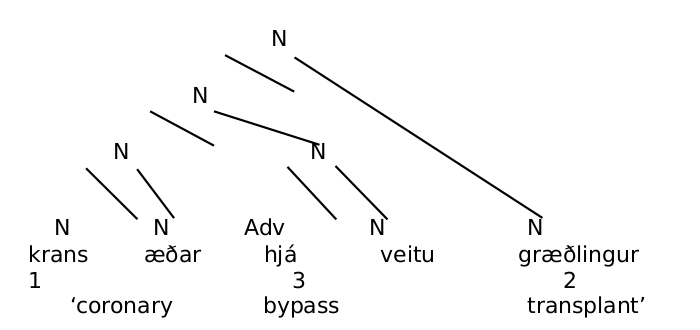
\includegraphics[width=\textwidth]{figures/bjarnadottir-stress.png}
\begin{forest} for tree={align=center}
 [N
  [ N 
    [ N
      [N\\krans,name=krans,inner sep=0pt, tier=bottom] [N\\æðar,tier=bottom] 
    ]
[ N
      [Adv\\hjá,name=hja, inner sep=0pt, tier=bottom,align=center] [N\\veitu, tier=bottom] 
    ]
]
[N\\græðlingur,name=graed, inner sep=0pt,align=center, tier=bottom]
]
\node[below=\baselineskip of krans.base west,inner sep=0pt] (1) {\strut 1};
\node[below right=2pt and 1em of 1.west,align=left] (coronary) {\strut `coronary};
\node[below=\baselineskip of hja.base west,inner sep=0pt] (3) {\strut 3};
\node[below right=2pt and 0em of 3.west,align=left] (bypass) {\strut bypass};
\node[below=\baselineskip of graed.base west,inner sep=0pt] (2) {\strut 2};
\node[below right=2pt and 0em of 2.west,align=left] (transplant) {\strut transplant'};
\end{forest}
%  [[[[N][N]][[Adv][N]][N]]] %>>> aligned with word forms:
%[[[[krans][æðar]] [[hjá][veitu]]] [græðlingur]] >>> and numbers:
%krans = 1; hjá = 3; græðlingur = 2: Please refer to Word document
\end{figure}

The compounds discussed in \sectref{sec:bjarnadottir:2} are assumed to conform to this basic \isi{stress pattern}, as do most of the PCIs in \sectref{sec:bjarnadottir:3.1}, but there is still insufficient research on the topic for an exact description of the exceptions. The complex structures in the PCIIs in \sectref{sec:bjarnadottir:3.2} below are more of a problem where stress is concerned, as the relatively simple rules of word stress do not apply to syntactic phrases as non-heads. Informally, the observation that the head of the PCIIs is stressed has been confirmed by native speakers, but proper experiments have not been carried out. The question whether these are indeed compounds phonologically therefore remains open, but comparative data from other languages shows that similar structures are analysed as PCs in those, as is the case in \citet{Trips2016} for \ili{English}. As most of the examples of PCIIs here are from written texts or transcriptions where the original sound files are unavailable, the question of phonology may be a moot point.

\subsection{Recursion}\label{sec:bjarnadottir:2.2}

Noun-noun compounds are by far the most common type of compounds in \ili{Icelandic}, and also the most structurally complex. As stated above, \ili{Icelandic} compounds are \isi{right-headed}, but the constituent structure in recursive compounds can be either left- or \isi{right-branching}, cf. examples in (\ref{ex:bjarnadottir:8}–\ref{ex:bjarnadottir:12}). Theoretically there is no limit to the length of compounds, and the classic example of this is the frequently quoted word in \REF{ex:bjarnadottir:3} \emph{Vaðlaheiðarvegavinnuverkfærageymsluskúrsútidyra\-ly\-klakippuhringur\textup{, where}} \emph{Vaðlaheiði \textup{is a compound place name.}} 

 \ea\label{ex:bjarnadottir:3} 
 \gll Vaðlaheiðar vega vinnu verk  færa geymslu skúrs úti dyra lykla kippu hringur\\
 V. road  works  work tools storage shed  out door key bunch ring\\
\glt ‘key ring of the key chain of the outer door to the storage tool shed of the road works on the Vaðlaheiði plateau’
\z 

{{Overlong compounds are apt to be split up in \ili{Icelandic}, using \isi{prepositional} phrases at need, and in reality more than seven constituents are rare \citep{Snædal1992,DaðasonEtAl2014}. The compound in \REF{ex:bjarnadottir:3} could be rephrased as} }

\ea
lyklakippuhringur fyrir útidyrnar á verkfærageymsluskúr vegavinnunnar á V\\
\glt ‘a key chain ring for the outside door of the tool storage shed of the roadworks on V.’
\z

In spite of the trend towards splitting, overlong compounds do sometimes occur, such as \emph{Norðausturatlantshafsfiskveiðinefndin} ‘The North East Atlantic Ocean Fisheries (lit. Fish-Catching) Committee’. Long PCs should therefore not cause a problem for Icelanders just because of their length, even if they are not common. 

\subsection{Inflection or compound markers?}\label{sec:bjarnadottir:2.3}

Nouns and adjectives as non-heads in \ili{Icelandic} compounds appear in different forms, i.e., as stems or inflectional forms, mostly \isi{genitive}. Dative non-heads are also found in compounds, as in \textit{gyðjumlíkur} ‘goddess\textsc{.n.fem.dat.pl} like\textsc{.adj}’ \citep{Bjarnadóttir2002}. A very limited number of non-head combining forms are also found, e.g., \textit{kven-} of the feminine noun \textit{kona} ‘woman’ where the regular non-head would be \textit{konu} (\textsc{gen.sg}) or \textit{kvenna} (\textsc{gen.pl}). Linking phonemes also occur, but these are rare,  with the proportion 0.005\% in 38,000 non-heads in compounds in \citealt{Bjarnadóttir19962005}. The discussion here will be limited to stems and \isi{genitive} forms as non-heads, as these are very frequent, whereas the other types are very rare.

The analysis of genitives as such in \ili{Icelandic} compounds is traditional in the \ili{Icelandic} \isi{grammatical} literature, dating back to Rasmus Christian Rask’s seminal work on \ili{Icelandic} grammar \citet{Rask1811}. According to this analysis, nouns as non-heads appear as stems or \isi{genitive} forms, singular or plural. Corresponding structures in \ili{Faroese} and some West \ili{Norwegian} dialects are analysed in the same manner in  \citet{Indriðason2014} and \citet{ThráinssonEtAl2004}

The nature of these genitives in \ili{Icelandic} compounds and the question whether these are true inflectional forms or linking phonemes are matters of debate, 
especially in theories that specify a strict ordering of \isi{derivation}, compounding and \isi{inflection}. The argumentation that these genitives are not a part of morphological structures, but attributes within noun phrases, is difficult to maintain for the following reasons: The \isi{stress pattern} described in \sectref{sec:bjarnadottir:2.1}. can be used to determine whether a structure is a compound or phrase, but additionally, basic \ili{Icelandic} word order provides clues, as \isi{genitive} attributes are usually placed after the nominal head in a sentence: \textit{bók Kristínar} ‘Kristín’s book’. The reverse order,  \textit{Kristínar bók}, is usually found with contrastive stress (cf. \citealt[92--96]{Thráinsson2007}). Furthermore, this analysis would leave almost half of the vocabulary, i.e. the so-called weak \isi{inflection}, unavailable for compound formation as these can never appear as stems in non-heads, cf. \sectref{sec:bjarnadottir:2.5}.\footnote{Further argumentation against level ordering or split morphology can be found in \ili{Icelandic} \isi{derivation}, as some suffixes can attach to \isi{genitive} non-heads: \textit{mannlegur} man\textsc{.n.masc.stem} -ly\textsc{.suff.adj} `human', \textit{mannslegur} man\textsc{.n.masc.gen.sg} -ly\textsc{.suff.adj} `manly', \textit{mannalegur} man\textsc{.n.masc.gen.pl} -ly\textsc{.suff.adj} `pompous, conceited' \citep{Bjarnadóttir19962005,Indriðason1994}.  
}

The case against analysing the \isi{genitive} non-heads in \ili{Icelandic} compounds as  compound markers or linking phonemes for \ili{Icelandic} also rests on the fact that
the non-heads appear as the correct \isi{genitive} forms, in spite of the complexity of the inflectional patterns. Inflectional variants are very common, and the paradigms in the DMII reflect this, with 594 inflectional patterns listed for the major word classes, i.e., nouns, adjectives, verbs, and adverbs (\citealt{Bjarnadóttir2012}). The reason for the high number of inflectional patterns in the DMII is that each paradigm contains all inflectional variants, i.e., a word is not assumed to belong to more than one inflectional class, as in the traditional classification in \ili{Icelandic} textbooks. The rampant variation found among \isi{genitive} singular inflectional forms is fully reflected in the form of the non-heads.

The non-heads appear as correct \isi{genitive} forms, as shown in all the examples in \sectref{sec:bjarnadottir:2.4}.\footnote{The exceptions are few, and can for the most part be explained by historical changes. These obsolete inflectional forms are only a feature of lexicalized compounds.} To give an example, the base word \textit{vegur} ‘way, road’ has the \isi{genitive} singular forms \textit{vegar} and \textit{vegs}, the first of which is much more frequent. Both \textit{-ar} and \textit{-s} appear in the non-heads of compounds, i.e., \textit{vegarendi} ‘end of road’, \textit{vegs\-auki} ‘increase of way’, i.e., ‘promotion’. (The \isi{genitive} plural \textit{vega} is also used in compounds: \textit{vegamót} ‘joint of roads, i.e., crossroads’). Compounds with the head \textit{vegur} can exhibit variants in the same way as the base word, but the crux of the matter is that these variants can be reflected in the non-heads of compounds as well, as in (\ref{ex:bjarnadottir:5}b–c). However, some compounds with the head \textit{vegur} only have \textit{-s} as a \isi{genitive} ending, thus exhibiting a different inflectional pattern from the base words, which is interesting in light of Lieber’s theories of percolation (\citeyear{Lieber1989}). This \isi{genitive} is always reflected in the non-heads of recursive compounds, as in \textit{útvegur} ‘out-way’, i.e., ‘fishing, fisheries’, and \textit{farvegur} ‘passage way’, i.e., ‘channel, course’ (\ref{ex:bjarnadottir:5}d–e). Underscoring marks the \isi{genitive} endings:
 
\ea%5
 \label{ex:bjarnadottir:5} 
\begin{xlist}
 \sn  \parbox{6cm}{Lemma}{ Gen.sg.}\\
\ex \parbox{6cm}{\textit{vegur} ‘way, road’} \textit{veg\underline{ar}, veg\underline{s}}\\
Compounds:\\
\textit{veg\underline{ar}endi} ‘end of road’\\
\textit{veg\underline{s}auki} ‘increase of way’, i.e., ‘promotion’

\ex \parbox{6cm}{\textit{reiðvegur} ‘(horse) riding road’} \textit{reiðveg\underline{ar}, reiðveg\underline{s}}\\
Compounds:\\ 
\textit{reiðveg\underline{ar}spotti} ‘stretch of riding road’\\
\textit{reiðveg\underline{s}framkvæmd} ‘riding road construction’

\ex \parbox{6cm}{\textit{Laugavegur} ‘pool way’ (street name)} \textit{Laugaveg\underline{ar}, Laugaveg\underline{s}}\\
Compounds:\\
\textit{Laugaveg\underline{s}apótek} ‘Pool Street Drug Store’\\
\textit{Laugarveg\underline{ar}ganga} ‘a walk along Pool Street’

\ex \parbox{6cm}{\textit{útvegur} ‘out-way’ (‘fisheries, fishing’)} \textit{útveg\underline{s}}\\
Compound:\\  
\textit{útveg\underline{s}þorp/ *útveg\underline{ar}þorp} ‘fisheries village’

\ex \parbox{6cm}{\textit{farvegur} ‘passage way’} \textit{farveg\underline{s}}\\
Compound:\\ 

\textit{farveg\underline{s}breyting/*farveg\underline{ar}breyting} ‘change of course’
\end{xlist}
\z\largerpage[2]

The conclusion is that \textit{-s} and \textit{-ar} are inflectional endings in \ili{Icelandic} compounds and not linking phonemes. This is directly opposite to the case of \ili{German}, where paradigmatically incorrect forms such as \textit{liebesbrief} ‘love letter’ are analysed as containing a prosodic \isi{marker}, here \textit{-s-}. With the correct feminine \isi{genitive}, the compound would be \textit{liebebrief} (Trips, personal communication).

The function of the \isi{genitive} in compounding is considered in \citet{Indriðason1999,Indriðason2014} in the light of the split morphology hypothesis \citep{Perlmutter1988} and the split \isi{inflection} theory \citep{Booij1994}, and his conclusion is that “the \isi{genitive} in \ili{Icelandic} compounds can formally be categorized as contextual \isi{inflection} but functionally as inherent \isi{inflection}. This dual role of the \isi{genitive} is unique and creates problems for the theories previously mentioned” \citep[30]{Indriðason2014}. The aim here is to present these so-called \isi{genitive} forms, to be able to compare them with the genitives in the PCs in \sectref{sec:bjarnadottir:3}, as these undoubtedly contain inflectional forms. The question is, then, whether the “ordinary” (i.e., non-phrasal) compounds contain true genitives. 

\subsection{Non-head in compounds: Nouns}\label{sec:bjarnadottir:2.4}

Examples of the different forms found in the non-heads of noun-noun compounds are shown in \REF{extab:bjarnadottir:2} (see \citealt{Bjarnadóttir2002}). These nouns are all written as continuous strings without hyphens. The lemma forms are shown in parentheses, as in \textit{naglrót} (\textit{n\underline{ö}gl+rót}).  Underscoring is used for \isi{genitive} endings and for emphasis, as in \textit{n\underline{ö}gl}, to mark the umlaut.


%Indentation: A + B, left margin. Numerals within A (1-4) and B (1-2): indented. 
%Letters %within numerals, indented 1 more step.
%Sequence: A.1.a, 2.b, 3.c, 4.d; B.1.e-j; 2.k-n
%cf. Word document


% \begin{table}
\ea
\label{extab:bjarnadottir:2}
% \caption{Form of non-head in noun-noun compounds}
Form of non-head in noun-noun compounds\\
\begin{xlist}
\exi{A.} Stem
\begin{xlist}
\exi{1.} Lemma form\footnote{Lemma form without \isi{nominative} ending where applicable, as in \textit{hest} for the masculine \textit{hestur}, subtracting the masculine \isi{nominative} ending \textit{-ur}.} 
\begin{xlist}
\exi{a.} 
	\gll orð myndun (orð+myndun) \\
	 word\textsc{.n.neut} formation\textsc{.n.fem}\\
	\glt ‘word formation’
\end{xlist}
\exi{2.} Without umlaut 
\begin{xlist}
\exi{b.} 
	\gll nagl rót (n\underline{ö}gl+rót) \\
	 nail\textsc{.n.fem} root\textsc{.n.fem}\\
	\glt ‘base of finger/toe-nail’ 
\end{xlist}\largerpage[1]
\exi{3.} With umlaut (rare) 
\begin{xlist}
\exi{c.} 
	\gll lög brot (l\underline{ö}g+brot) \\
     law\textsc{.n.neut.pl} breaking\textsc{.n.neut}\\
	\glt ‘infraction of law’
\end{xlist}
\exi{4.} Irregular (rare change in stem)
\begin{xlist}
\exi{d.} 
	\gll mann tal (maður+tal) \\
	  man\textsc{.n.masc} count\textsc{.n.neut}\\
	\glt ‘census’
\end{xlist}
\end{xlist}
\exi{B.} Inflectional forms
\begin{xlist}
\exi{1.} Genitive singular 
\begin{xlist}
\exi{e.} 
	\gll borð\underline{s} horn (borð+horn) \\
	 table\textsc{.n.neut.gen.sg} corner\textsc{.n.neut}\\
	\glt ‘corner of a table’

\exi{f.} 
	\gll hund\underline{s} haus (hundur+haus) \\
	 dog\textsc{.n.masc.gen.sg} head\textsc{.n.masc}\\
	\glt ‘head of a dog’

\exi{g.} 
	\gll katt\underline{ar} haus (k\underline{ö}ttur+haus)  \\
	 cat\textsc{.n.masc.gen.sg} head\textsc{.n.masc}\\
	\glt ‘head of a cat’

\exi{h.} 
	\gll penn\underline{a} strik (penni+strik){\rmfnm}  \\
	 pen\textsc{.n.masc.gen.sg} stroke\textsc{.n.neut}\\
\footnotetext{The use of stems is limited in some inflectional classes, cf. \sectref{sec:bjarnadottir:2.5}.}
\glt ‘stroke of a pen’ 

\exi{i.} 
	\gll per\underline{u} tré  (pera+tré) \\
	 pear\textsc{.n.fem.gen.sg} tree\textsc{.n.neut}\\
	\glt ‘pear tree’

\exi{j.} 
	\gll bók\underline{ar} kápa (bók+kápa) \\
	 book\textsc{.n.fem.gen.sg} coat\textsc{.n.fem}\\
	\glt ‘dust jacket’
\end{xlist}
\exi{2.} Genitive plural\footnote{The \isi{genitive} plural of all nouns ends in -\textit{a} (or -\textit{na} for some feminine and neuter nouns).}
  \begin{xlist}
\exi{k.} 
	\gll orð\underline{a} bók (orð+bók)\\
	 word\textsc{.n.neut.gen.pl} book\textsc{.n.fem}\\
	\glt ‘dictionary’

\exi{l.} 
	\gll bíl\underline{a} stæði (bíll+stæði) \\
	 car\textsc{.n.masc.gen.pl} place\textsc{.n.neut}\\
	\glt ‘car place, parking lot’

\exi{m.} 
	\gll bók\underline{a} búð (bók+búð) \\
	 book\textsc{.n.fem.gen.pl} store\textsc{.n.fem}\\
	\glt ‘book shop’

\exi{n.} 
	\gll dúf\underline{na} kofi (dúfa+kofi)\textsuperscript{8} \\
	 pigeon\textsc{.n.fem.gen.pl} hut\textsc{.n.masc}\\
	\glt ‘pigeon hut’
\end{xlist}
\end{xlist}
\end{xlist}
\z 
% \end{table}


The \isi{genitive} forms of the non-head in compounds are in accordance with the correct genitives, as they occur in the paradigms in the DMII. To give examples, the genitives of the masculine nouns \textit{hundur} ‘dog’ and \textit{köttur} ‘cat’ are \textit{hunds}/*\textit{hundar} and \textit{kattar}/*\textit{kötts}, and always appear as such when the \isi{genitive} is used in the non-heads of the compounds of these words (cf. B.1.f and g in \REF{extab:bjarnadottir:2}). A choice of identical linking phonemes to the correct \isi{genitive} endings is less than convincing, especially as the choice of endings on individual words is for the most part idiosyncratic. PCs with \isi{genitive} phrases as non-heads also invariably contain the correct \isi{genitive} forms. 


The choice of stem or inflected form seems to be arbitrary for compounds where the non-head is a base noun, i.e., not a compound (\citealt{Bjarnadóttir1995}), with the exceptions discussed below (this section). The compounds \textit{bóksala} and \textit{bóka\-búð} shown in \REF{ex:bjarnadottir:6} thus contain the stem and the \isi{genitive} plural of the word \textit{bók} ‘book’ as non-heads without any discernible reason for the difference, as the compounds are semantically identical with synonyms as heads. The distribution is not phonetically conditioned either, as seen in \textit{blekborði (k+b)} ‘ink strip’ (cf. \textit{bókabúð}), and \textit{bókasafn} (ka+s) ‘book museum’, i.e., ‘library’ (cf. \textit{bóksala}) occurring freely on morpheme boundaries:


\ea%6
 \label{ex:bjarnadottir:6} 
\ea bók\textsc{.n.fem.stem} sala\textsc{.n.fem} ‘book shop’

\ex  bóka\textsc{.n.fem.gen.pl} búð\textsc{.n.fem} ‘book shop’
\z
\z

The choice of stem or \isi{genitive} construction may be arbitrary in non-recursive compounds, as in \REF{ex:bjarnadottir:6}, but it turns out that it is not free, i.e., the form itself can be lexicalized, so to speak, as users will only accept the expected variant, thus \textit{bóksala, bókabúð} vs. \textit{*bókasala, *bókbúð}. The same can apply to the choice between \isi{genitive} singular and plural, which is often not semantically significant, as in (\ref{ex:bjarnadottir:7}a–b) where \textit{barns}/\textit{barna} can refer to one or more children.\footnote{The difference between \isi{genitive} singular and plural can be significant, as in \textit{bróðursonur} `brother's\textsc{.n.masc.gen.sg} son\textsc{.n.masc.sg}' (`the son of (your) brother'), \textit{bróðursynir} `brother's\textsc{.n.masc.gen.sg} sons\textsc{.n.masc.pl}' (`the sons of (your) brother'), and \textit{bræðrasynir} `brothers'\textsc{.n.masc.gen.pl} sons'\textsc{.n.masc.pl} (`the sons of (your) brothers'). The compound \textit{bræðrasonur} `brothers'\textsc{.n.masc.gen.pl} son'\textsc{.n.masc.sg} (`the son of (your) brothers') is not found. Some nouns exhibit agreement of number between non-head and head, as in the singular \textit{mannsnafn} `persons'\textsc{.n.masc.gen.sg} name' \textsc{.n.neut.sg} (i.e., `Christian name') vs. the plural \textit{mannanöfn} `persons' \textsc{.n.masc.gen.pl} names\textsc{.n.neut.pl} (i.e., `Christian names'). It is unclear how extensive number agreement of this type is in compounds and the topic awaits further research.}


\ea%7
 \label{ex:bjarnadottir:7} 
\ea
\gll barns meðlag\\
child\textsc{.n.neut.gen.sg} support\textsc{.n.neut}\\
\glt ‘child support’ (paid by parent)

\ex
\gll barna lífeyrir\\
child\textsc{.n.neut.gen.pl} support\textsc{.n.masc.pl}\\
\glt ‘child support’ (paid by state, etc.)

\ex
\gll  barns vagga\\
child\textsc{.n.neut.gen.sg} crib\textsc{.n.fem}\\
\glt ‘baby’s crib’

\ex
\gll  barna rúm\\
child\textsc{.n.neut.gen.pl} bed\textsc{.n.neut}\\
\glt ‘baby’s cot’
\z
\z

The choice between stem and \isi{genitive} appears to be less free in recursive compounding, with \isi{left-branching} compounds ([[N N] N]) tending to result in \isi{genitive} constructions \citep{Jónsson1984}, when the corresponding non-recursive compound does not, as in the pairs \textit{skrifborðsfótur} \REF{ex:bjarnadottir:8a} and \textit{borðfótur} \REF{ex:bjarnadottir:8b}, and \textit{olíuverðshækkun} \REF{ex:bjarnadottir:8c} and \textit{verðhækkun} \REF{ex:bjarnadottir:8d}:


\ea%8
 \label{ex:bjarnadottir:8} 
\ea  \label{ex:bjarnadottir:8a}
\gll {\ob}skrif borðs] fótur\\
   write\textsc{.n.neut.stem} desk\textsc{.n.neut.gen.sg} leg\textsc{.n.masc}\\
\glt ‘writing desk leg’

\ex  \label{ex:bjarnadottir:8b}
\gll borð fótur \\
 desk\textsc{.n.neut.stem} leg\textsc{.n.masc}\\
\glt ‘desk leg’

\ex  \label{ex:bjarnadottir:8c}
\gll {\ob}olíu verðs] hækkun\\
 oil\textsc{.n.fem.gen.sg} price\textsc{.n.neut.gen.sg} rise\textsc{.n.fem}\\
\glt ‘rise in oil price’

\ex  \label{ex:bjarnadottir:8d}
\gll verð hækkun \\
 price\textsc{.n.neut.stem} rise\textsc{.n.fem}\\
\glt ‘price rise’
\z
\z

Left-branching recursive compounds with stems of compounds as non-heads do also occur, although they are much rarer than the corresponding \isi{genitive} constructions. These are of two kinds, i.e., with a stem compound as first part of the non-head [[N.\textsc{stem} N]\textsc{stem} N] (cf. \textit{saltfiskútflutningur}, \ref{ex:bjarnadottir:9b}),  and with a \isi{genitive} compound as first part of the non-head [[N\textsc{.gen} N]\textsc{stem} N] (cf. \textit{fjárhúsdyr}, \ref{ex:bjarnadottir:9c}):

\ea%9
 \label{ex:bjarnadottir:9}
\ea  \label{ex:bjarnadottir:9a}
\gll {\ob}kú fisk] plógur\\
 	  cow\textsc{.n.fem.stem} fish\textsc{.n.masc.stem} plough\textsc{.n.masc}\\
\glt ‘ocean quahog plough’

\ex \label{ex:bjarnadottir:9b}
\gll {\ob}salt fisk] útflutningur\\
     salt\textsc{.n.neut.stem} fish\textsc{.n.masc.stem} export\textsc{.n.masc}\\
\glt ‘salt fish export’

\ex \label{ex:bjarnadottir:9c}
\gll {\ob}fjár hús] dyr\\
      sheep\textsc{.n.neut.gen.sg} house\textsc{.n.neut.stem} door\textsc{.n.fem.pl}\\
\glt ‘sheep house door’

\ex \label{ex:bjarnadottir:9d}
\gll {\ob}betrunar hús] vist\\
    betterment\textsc{.n.fem.gen.sg} house\textsc{.n.neut.stem} stay\textsc{.n.fem.sg}\\
\glt ‘stay in jail’ 

\ex \label{ex:bjarnadottir:9e}
\gll {\ob}rentu kammer] bréf\\
   rent\textsc{.n.fem.gen.sg} chamber\textsc{.n.neut.stem} letter\textsc{.n.neut.sg}\\
\glt ‘letter from the (Danish) ministry of finance’ (\textit{renta}: ‘rent, interest’)
\z
\z

The observation in \citealt{Jónsson1984} of the strong tendency towards \isi{genitive} in compound non-heads holds for the most part, but stem compounds as in (\ref{ex:bjarnadottir:9}a–b) do also exist in compound non-heads, sometimes even as variant forms, as in \REF{ex:bjarnadottir:9b} \textit{saltfiskútflutningur} [[N\textsc{.stem} N]\textsc{.stem} N] where the corresponding \textit{saltfisk}\textbf{\textit{s}}\textit{útflutn\-ing\-ur} [[N\textsc{.stem} N]\textsc{gen} N] is also found.\footnote{In this case the stem compound \textit{saltfiskútflutningu}r seems to be much more common than the \isi{genitive} compound \textit{saltfisksútflutningur}. The frequency on timarit.is (The National Library’s corpus of newspapers and journals) is 372\slash 104.} The compounds in (\ref{ex:bjarnadottir:9}c–d) are more problematic, as these contain a stem ending in -\textit{s} where the \isi{genitive} ending would also be an -\textit{s}. The syllables containing the \isi{genitive} are unstressed, moreover, as can be inferred from \figref{fig:bjarnadottir:1} above, and the difference in vowel length normally occurring in such genitives (i.e., \textit{hús} vs. \textit{húss}) may thus not be discernible \citep{Árnason2011}. This could therefore be a matter of spelling, although the \isi{genitive} \textit{-s} is usually preserved in such cases. The compound in \REF{ex:bjarnadottir:9e}, \textit{rentukammerbréf},\largerpage contains an undisputed \isi{genitive} construction in \textit{rentu}\textsc{.n.gen.sg.}\textit{kammer}, but the first part is in fact a weak feminine noun which can never appear as a stem, as is the case in the word \textit{olía} in \REF{ex:bjarnadottir:8c} (cf. \sectref{sec:bjarnadottir:2.5}). The evidence for the construction [[N\textsc{.gen} N]\textsc{stem} N] therefore does not seem to be very strong.

Right-branching recursive compounds do not exhibit similar restrictions as the \isi{left-branching} ones do, as stem constructions and \isi{genitive} constructions mix freely:


%I + IV. to the left, a-l indented within these: I.a-c; II.d-f; III.g-i; IV.j-l
\ea%10
 \label{ex:bjarnadottir:10} 
\begin{xlist}
 
\exi{I.}{} [N.STEM [N.STEM N]]

\begin{xlist}
\exi{a.}
\gll {\ob}stál [borð búnaður]]\\
 steel\textsc{.n.neut.stem} table\textsc{.n.neut.stem} equipment.\textsc{n.masc.sg}\\
\glt ‘steel cutlery’

\exi{b.}
\gll {\ob}stíl [hug sjón]] \\
 style\textsc{.n.masc.stem} mind\textsc{.n.masc.stem} vision\textsc{.n.fem.sg}\\
\glt ‘ideal of style’

\exi{c.}
\gll {\ob}her [flug maður]] \\
 army\textsc{.n.masc.stem} flight\textsc{.n.neut.stem} man\textsc{.n.masc.sg}\\
\glt ‘military pilot’
\end{xlist}

\exi{II.}{}  [N.GEN. [N.STEM N]]
\begin{xlist}
\exi{d.}
\gll {\ob}togara [sjó maður]] \\
 trawler\textsc{.n.masc.gen.sg} sea\textsc{.n.masc.stem} man\textsc{.n.masc.sg}\\
\glt ‘trawler fisherman’

\exi{e.}
\gll {\ob}bómullar  [hand klæði]] \\
 cotton\textsc{.n.fem.gen.sg} hand\textsc{.n.fem.stem} cloth\textsc{.n.neut}\\
\glt ‘cotton towel’

\exi{f.}
\gll {\ob}atvinnu  [flug maður]] \\
 profession\textsc{.n.fem.gen.sg} flight\textsc{.n.neut.stem} man\textsc{.n.masc.sg}\\
\glt ‘professional pilot’
\end{xlist}
\exi{III.}{}  [N.STEM [N.GEN. N]]
\begin{xlist}
\exi{g.} \label{ex:bjarnadottir:10g}
\gll {\ob}plast [hnífa par]] \\
 plastic\textsc{.n.neut.stem} knife\textsc{.n.masc.gen.pl} pair\textsc{.n.neut.sg}\\
\glt ‘plastic cutlery’ (usually set of knife, fork \& spoon)\footnote{The spoon may be optional, but this is emphatically not a pair of two plastic knives, i.e., not [[\textit{plast hnífa}] \textit{par}].}

\exi{h.}
\gll {\ob}hör [vasa klútur]] \\
 linen\textsc{.n.masc.stem} pocket\textsc{.n.masc.gen.sg} cloth\textsc{.n.masc}\\
\glt ‘linen handkerchief’

\exi{i.}
\gll {\ob}grunn [fjár festing]] \\
 base\textsc{.n.masc.stem} capital\textsc{.n.neut.gen.sg} fastening\textsc{.n.fem}\\
\glt ‘basic investment’
\end{xlist}
\exi{IV.}{} 	[N.GEN.[N.GEN. N]]
\begin{xlist}
\exi{j.}
\gll {\ob}biskups  [skjala safn]]\\
 bishop\textsc{.n.masc.gen.sg} document\textsc{.n.neut.gen.pl} collection\textsc{.n.neut}\hspace*{-2mm}\\
\glt ‘archives of the bishop’

\exi{k.}
\gll {\ob}blúndu [vasa klútur]]  \\
 lace\textsc{.n.fem.gen.sg} pocket\textsc{.n.masc.gen.sg} cloth\textsc{.n.neut}\\
\glt ‘lace handkerchief’

\exi{l.}
\gll {\ob}hernaðar [leyndar mál]] \\
 warfare\textsc{.masc.gen.sg} secret\textsc{.n.fem.gen.sg} matter\textsc{.n.neut}\\
\glt ‘military secret’
 \end{xlist}
\z
\z

The examples in (\ref{ex:bjarnadottir:10}g--i) are critical in respect to theories with any kind of ordering of stem and \isi{genitive} compounds. Imposing a \isi{left-branching} structure on (\ref{ex:bjarnadottir:10}g) would change the meaning of \textit{plasthnífapar} from ‘a set of knife and fork made from plastic’ to ‘a pair of knives ...’. Posing different structures for (\ref{ex:bjarnadottir:10}h) \textit{hörvasa\-klútur} ‘linen handkerchief’ and (\ref{ex:bjarnadottir:10}k) \textit{blúnduvasaklútur} ‘lace handkerchief’ and the corresponding set of towels in (\ref{ex:bjarnadottir:11}a–b) seems semantically counterintuitive:

\ea%11
 \label{ex:bjarnadottir:11} 
 
\ea 
\gll {\ob}hör [hand klæði]] \\
 linen\textsc{.n.masc.stem}  hand\textsc{.n.neut.stem} cloth\textsc{.n.masc}\\
\glt ‘linen towel’

\ex
\gll {\ob}bómullar [hand klæði]]  \\
 cotton\textsc{.n.fem.gen.sg} hand\textsc{.n.neut.stem} cloth\textsc{.n.masc}\\
\glt ‘cotton towel’

\ex
\gll {\ob}hör [vasa klútur]]  \\
 linen\textsc{.n.masc.stem} pocket\textsc{.n.masc.gen} cloth\textsc{.n.masc}\\
\glt ‘linen handkerchief’

\ex
\gll {\ob}blúndu [vasa klútur]]  \\
 lace\textsc{.n.fem.gen.sg} pocket\textsc{.n.masc.gen} cloth\textsc{.n.masc}\\
\glt ‘lace handkerchief’
\z
\z\largerpage[2]

An explanation based on the fact that \textit{handklæði} and \textit{vasaklútur} are lexicalized compounds will not suffice either, as fully productive compounds with these structures are easily made:\footnote{These compounds are nonce formations. All nonce formations in this text are clearly marked as such.}

\ea%12
 \label{ex:bjarnadottir:12} 
\ea 
\gll {\ob}plast [penna dallur]]\\
 plastic\textsc{.n.neut.stem} pen\textsc{.n.masc.gen} tub\textsc{.n.masc}\\
\glt ‘plastic pen container’

\ex
\gll {\ob}postulíns [penna dallur] \\
 porcelain\textsc{.n.neut.gen.sg} pen\textsc{.n.masc.gen} tub\textsc{.n.masc}\\
\glt ‘porcelain pen container’
\z
\z

The modifiers \textit{plast} and \textit{postulín} refer to the material of the container, not the pens stored in it.

\subsection{Restriction of the use of stems as non-heads}\label{sec:bjarnadottir:2.5}

Words from some inflectional classes can never appear as stems in compounds and there the \isi{genitive} forms are always used. This applies to the so-called weak \isi{inflection} of feminine and masculine nouns, e.g., feminine nouns ending in \textit{-a} in the \isi{nominative} singular, as in \textit{olía} in \textit{olíuverðshækkun} ‘a rise in the price of oil’ in \REF{ex:bjarnadottir:8c}, and masculine nouns ending in \textit{-i} in the \isi{nominative} singular, as in \textit{vasi} in \textit{vasaklútur} ‘(pocket) handkerchief’ in \REF{ex:bjarnadottir:11}. Words of this type are very numerous, as seen in the DMII which contains 27,381 non-compounds. Out of a total of 13,116 masculine and feminine nouns, 6,540 belong to the weak \isi{inflection}, or just under 50\%.

This fact should not be forgotten when the proportions of stem compounds and \isi{genitive} compounds are considered, as the result is that a large proportion of the vocabulary is unavailable for stem compounds.\footnote{There are a few exceptions where the combining forms of weak masculine nouns are stems, e.g., \textit{sím-} for \textit{sími} `telephone', e.g., \textit{símhringing} ‘telephone call’, where \textit{síma-} would be expected. These cases are extremely rare and most compounds with \textit{sími} have the \isi{genitive} non-head \textit{síma}, e.g., \textit{símasamband} ‘telephone connection’.} The consequences of this for any kind of ordering based on the difference of stems and inflected non-heads in compounds are unclear, but the option of specifying that half of the vocabulary is unavailable at any given level seems counter-intuitive. 

\subsection{Non-heads in compounds: Adjectives} \label{sec:bjarnadottir:2.6}

Adjectives as non-heads of compounds exhibit similar variants as nouns do, i.e., stems (\textit{lítil} ‘small’ in \textit{lítilmenni} ‘insignificant character’ (A.b in \ref{extab:bjarnadottir:3}) and genitives (\textit{lítils} in \textit{lítilsverður} ‘insignificant’ (B.c in \ref{extab:bjarnadottir:3})). Internal \isi{inflection} is also found in adjectives as non-heads in compounds with nominal heads, where agreement of  gender, case, and number is exactly the same within the compounds as in \isi{syntax}, 
as in the \isi{nominative} \textit{litlifingur} ‘little finger, pinkie’, where the ending \textit{-i-} in the non-head is a portmanteau \isi{adjectival} ending for masculine, singular, \isi{nominative}, definite, and the accusative \textit{litlafingur}, where the ending \textit{-a-} is a portmanteau \isi{adjectival} ending for masculine, singular, accusative, definite, cf. (\ref{extab:bjarnadottir:3}C.). A comparison of agreement within a compound and in \isi{syntax} is shown in \tabref{tab:bjarnadottir:4}.

%Alignment: A, B, C to the left, indentation: A.a-b; B.c-d; C.e-g
%%please move \begin{table} just above \begin{tabular
% \begin{table}
\ea
\label{extab:bjarnadottir:3}
{\textit{Form of adjectives as non-heads of compounds}}
% \caption{\textit{Form of adjectives as non-heads of compounds}}
\begin{xlist}
\exi{A.} Stem 
\begin{xlist}
	\exi{a.}
	\gll blá ber  (blár+ber)\\
	 blue\textsc{.adj.stem} berry\textsc{.n.neut}\\
	\glt ‘blueberry’

	\exi{b.}
	\gll lítil menni (lítill+-menni (\textit{menni}=bound form)) \\
	 small\textsc{.adj.stem} man\textsc{.n.masc}\\
	\glt ‘insignificant character’
\end{xlist}
\exi{B.} Inflection, \isi{genitive} (indefinite)
\begin{xlist}
	\exi{c.}
	\gll lítils verður (lítill+verður) \\
	 small\textsc{.adj.gen.sg.indef} worthy\textsc{.adj}\\
	\glt ‘insignificant’

	\exi{d.}
	\gll sjúkra hús (sjúkur+hús) \\
	 sick\textsc{.adj.gen.pl.indef} house\textsc{.n.neut}\\
	\glt ‘hospital’
\end{xlist}
\exi{C.} Inflection, internal\footnote{Degree, as shown in the superlative \textit{hæstiréttur} ‘supreme court’ in \REF{extab:bjarnadottir:3} (C)g, is not an instance of internal \isi{inflection} but a contextual feature \citep[21]{Indriðason2014}. Internal \isi{inflection} in the comparative only appears in place names in Modern \ili{Icelandic} and is not shown here.}
\begin{xlist}
\exi{1.} Positive degree
\begin{xlist}
	\exi{e.}
	\gll litli fingur  \\
	 little\textsc{.adj.masc.def} finger\textsc{.n.masc.indef}\\
	 
	 (\textit{lítill+fingur}; Acc. \textit{litlafingur})
	\glt ‘pinkie, little finger’

	\exi{f.}
	\gll Bratta brekka  \\
	 steep\textsc{.adj.fem.def} hill\textsc{.n.fem}\\
	 
	 (\textit{brattur+brekka}; Acc. \textit{Bröttubrekku}) 
	\glt ‘Steep Hill’ (placename)
\end{xlist}
 \exi{2.} Superlative 
\begin{xlist}
	\exi{g.}
	\gll hæsti réttur  \\
	 highest\textsc{.adj.masc.sup.def} court\textsc{.n.masc.indef}\\
	 
	 (\textit{hár+réttur}; Acc. \textit{hæstarétt}) 
	\glt ‘supreme court’ 
\end{xlist}
\end{xlist}
\end{xlist}
\z

Definiteness is an inflectional feature of \ili{Icelandic} adjectives (cf. \tabref{tab:bjarnadottir:4}). The genitives in B in \REF{extab:bjarnadottir:3} are indefinite forms, but \isi{adjectival} non-heads in C in \REF{extab:bjarnadottir:3} are always definite, irrespective of the definiteness of the compound as a whole. For explanation, \tabref{tab:bjarnadottir:4} contains the paradigms for the noun phrase \textit{lítill fingur} ‘little finger’ in column 1 and 2, and the internal \isi{inflection} for the compound \textit{litlifingur} ‘pinkie’ in the compound in column 3. 

\begin{table}
\caption{Paradigms for noun phrases and internal adjectival inflection}
\label{tab:bjarnadottir:4}

\begin{tabularx}{\textwidth}{>{\scshape}lXXX}
\lsptoprule
\textup{singular} & indefinite & definite & compound\\
\midrule
nom. &  {lítill fingur} &  {litl}\textbf{{i}}  {fingurinn} 
&  {litl}\textbf{{i}}{fingur}\\
acc. &  {lítinn fingur} &  {litl}\textbf{{a}}  {fingurinn} 
&  {litl}\textbf{{a}}{fingur}\\
dat. &  {litlum fingri} &  {litl}\textbf{{a}}  {fingrinum} 
&  {litl}\textbf{{a}}{fingri}\\
gen. &  {lítils fingurs} &  {litl}\textbf{{a}}  {fingursins} 
&  {litl}\textbf{{a}}{fingurs}\\
\tablevspace
\textup{plural} &  &  & \\
\midrule
nom. &  {litlir fingur} &  {litl}\textbf{{u}}  {fingurnir} 
&  {litl}\textbf{{u}}{fingur}\\
acc. &  {litla fingur} &  {litl}\textbf{{u}}  {fingurna} 
&  {litl}\textbf{{u}}{fingur}\\
dat. &  {litlum fingrum} &  {litl}\textbf{{u}}  {fingrunum} 
&  {litl}\textbf{{u}}{fingrum}\\
gen. &  {lítilla fingra} &  {litl}\textbf{{u}}  {fingranna} 
&  {litl}\textbf{{u}}{fingra}\\
\lspbottomrule
\end{tabularx}
\end{table}

Note that the internal \isi{inflection} in the compound in column 3 in \tabref{tab:bjarnadottir:4} is identical to the definite inflectional form in column 2. This is in fact the case in all compounds of this type in the DMII, but the construction is not very common, except in place names. The form of the compound is indefinite, however, and the cliticized definite article can be attached, in the same manner as in other nouns, as seen in the examples in \REF{ex:bjarnadottir:13}:

\ea%13
 \label{ex:bjarnadottir:13} 
\ea
\gll Hann braut litlafingur,  held ég.\\
 he broke littlefinger\textsc{.n.masc.acc.sg.indef}, think I\\
\glt ‘He broke a pinkie, I think.’

\ex
\gll Hann braut á sér ~ litlafingurinn\\
 he broke on himself  (the) littlefinger\textsc{.n.masc.acc.sg.def}\\
\glt ‘He broke his pinkie.’

\ex
\gll Litlifingurinn brotnaði.\\
 the-littlefinger\textsc{.n.masc.nom.sg.def} broke\\
\glt ‘The pinkie broke/was broken.’
\z
\z

The \isi{genitive} constructions with \isi{adjectival} non-heads have direct counterparts in 
PCs, in the same manner as nouns. They are, however, quite rare, cf. \sectref{sec:bjarnadottir:3.1.2}.

\subsection{The relevant features of non-phrasal compounding for PCs}

The salient points in this section in connection with the PCs discussed in the next section are these:

\begin{itemize}
\item 
Genitive non-heads are one of two basic options in forming \ili{Icelandic} non-phrasal compounds. The other main option is to have non-head stems. Genitive non-heads are also found in PCs, as will be discussed in \sectref{sec:bjarnadottir:3}.
\end{itemize}
\begin{itemize}
\item 
The distribution of genitives and stems as non-heads in compounds is partly dependent on the inflectional class of the non-head, as masculine and feminine words from the so-called weak \isi{inflection} cannot appear as stems in compounds, with exceptions mentioned in Footnote 13. Right-branching compounds with \isi{genitive} non-heads in a lower node than stem non-heads are quite common. Therefore, it is difficult to maintain strict ordering of stems and genitives as non-heads of compounds for \ili{Icelandic}.
\end{itemize}
\begin{itemize}
\item 
The inflected non-heads are in accordance with the “correct” \isi{inflection} of the respected unbound forms. This also applies in PCs.
\end{itemize}
\begin{itemize}
\item 
The internal \isi{inflection} of \isi{adjectival} non-heads could perhaps be analysed as a phrase-to-word conversion. \sectref{sec:bjarnadottir:3.1.4} contains PCs with \isi{prepositional} phrases which could also be analysed as phrase to word conversion, as could some of the PCII structures in \sectref{sec:bjarnadottir:3.2}, cf. also Footnote 16. The process of phrase to word conversion (or nominalization) will not be discussed in any detail, as the necessary research is not available.
\end{itemize}

\section{Phrasal compounds}\label{sec:bjarnadottir:3}

Below, \ili{Icelandic} PCs are divided into two groups. The first group (\sectref{sec:bjarnadottir:3.1}) contains common words which are not stylistically marked in any way, some of which are attested from medieval times to the present day. This group of PCs contains \isi{genitive} noun phrases and \isi{prepositional} phrases as modifiers of nouns, as in \tabref{tab:bjarnadottir:5}. (Examples of all constructions are given in the following sections.)

%Check formatting
\begin{table}
  \caption{Phrasal Compounds I, from lexicographic sources}
  \label{tab:bjarnadottir:5}
\begin{tabular}{lll}
\lsptoprule
  a. &NP.GEN. + N 	&Phrase internal agreement \\
  b. &AdjP.GEN. + N 	&Phrase internal agreement (rare)\\
  c. &PP + N 		&Case assignment by preposition\\
\lspbottomrule
  \end{tabular}
\end{table}

The second group contains more complex PCs, mainly found in informal writing and in speech. The structures are variable, up to full main clauses. The evidence for some of the structures is weak, down to single examples. The classification in \sectref{sec:bjarnadottir:3.2} reflects this. It should be noted that the more traditional PC types shown in \tabref{tab:bjarnadottir:5} also appear in the more informal texts used as sources for PCIIs.

%Check formatting
\begin{table}\caption{Phrasal Compounds II, from the web, etc.\label{tab:bjarnadottir:6}}
\begin{tabular}{lll}\lsptoprule 
  a. &[N.NOMINATIVE + PP]NP + N 		&Case assignment by preposition\\
  b. &Miscellaneous non-predicates:  &AdjP, AdvP, negation, etc. \\
  c. &Predicates: 					&Imperatives, questions, finite S, etc.\\\lspbottomrule
\end{tabular}
\end{table}

As the second type of PCs is very much a feature of informal speech and text, the spelling tends to be varied. In fact, \ili{Icelandic} spelling rules do not include any indication of the correct form in these cases.\footnote{The only indication is the spelling of compounds containing multiword first parts of foreign origin, such as the translation of \textit{New York City}, i.e., \textit{New York-borg}, where the spelling rules place a hyphen before the compound head \textit{borg} `city'. The space in \textit{New York} from the \ili{English} original is maintained. Judging by all the mistakes made, this spelling rule seems to be hard to learn, and extending it to phrasal compounds seems to be counter-intuitive as spelling as in \REF{ex:bjarnadottir:14f} (\textit{munn við munn-aðferð}) is hardly ever found.} The PCs are therefore a free-for-all in \ili{Icelandic} spelling, which makes them very difficult to extract automatically from text. The examples in \REF{ex:bjarnadottir:14} show spelling variations with different quotation marks, hyphenation, and spaces, found in data from a corpus of \ili{Icelandic} websites, \textit{Íslenskur orðasjóður} \citep{HallsteinsdóttirEtAl2007}:


% check simple and double quotes in example?
% KB: The point is that these are not standardized; these are direct quotes, quotation marks and all. Please leave them as they are.

\ea%14
 \label{ex:bjarnadottir:14} 
\ea \label{ex:bjarnadottir:14a} \parbox{5cm}{\textit{„allt eða ekkert“ aðferðin}} ‘the all or nothing method’
\ex \label{ex:bjarnadottir:14b} \parbox{5cm}{\textit{“allt eða ekkert” dæmi}} ‘[an] all or nothing example’
\ex \label{ex:bjarnadottir:14c} \parbox{5cm}{\textit{‘allt eða ekkert’ týpa}} ‘[an] all or nothing type’, i.e., ‘guy’
\ex \label{ex:bjarnadottir:14d} \parbox{5cm}{\textit{allt eða ekkert dæmi}} ‘[an] all or nothing example’
\ex \label{ex:bjarnadottir:14e} \parbox{5cm}{\textit{munn-við-munn-öndun}} ‘[a] mouth to mouth breathing’
\ex \label{ex:bjarnadottir:14f} \parbox{5cm}{\textit{munn við munn-aðferð}} ‘[a] mouth to mouth method’
\ex \label{ex:bjarnadottir:14g} \parbox{5cm}{\textit{allt-eða-ekkert hugsunarháttur}}  ‘[an] all or nothing way of thinking’
\z
\z

The possible spelling varieties are not exhausted in this search, but at present, tools for an automatic search do not exist. No attempt is made here to normalize the spelling in these examples, resulting in strange quotation marks at times.

The PCs discussed here are a subset from a collection of over 200,000 compounds compiled by the author over a period of over 30 years. The sources are mostly the same as those for the DMII mentioned above (\citealt{Bjarnadóttir19962005,Bjarnadóttir2012}), and the analysis contains lemmatization and full analysis of the con\-stit\-u\-ents of the compounds. This resource returned ca. 700 PCs, almost all of which are PCIs. In addition, ca. 200 PCs from the web, from blogs, social media, radio, and TV, were collected from \textit{Íslenskur orðasjóður}, and from miscellaneous sources, personal communication, etc. Finding data for PCIIs turned out to be difficult, because of unstandardized spelling. The remainder of this section contains a classification of these 900 PCs.

\subsection{Phrasal compounds I}\label{sec:bjarnadottir:3.1}

\subsubsection{Genitive noun phrase and nominal head}\label{sec:bjarnadottir:3.1.1}

Genitive noun phrases with adjectives are common in any genre as non-heads of compounds.  There is full agreement of gender, case and number within the noun phrases, as in \textit{Góðrarvonarhöfði} ‘Cape of Good Hope’ \REF{ex:bjarnadottir:15c}. where the adjective \textit{góður} ‘good’ agrees in gender with the feminine noun \textit{von} ‘hope’, and both agree in case (gen.), and number (sg.). The head \textit{höfði} ‘cape’ is a masculine noun.

\ea%15
 \label{ex:bjarnadottir:15} 
\ea \label{ex:bjarnadottir:15a} 
\gll {\ob}hálfs mánaðar]\textsc{np}  blað \\
 half\textsc{.adj.masc.gen.sg} month\textsc{.n.masc.gen.sg} paper\textsc{.n.neut.sg}\\
\glt ‘biweekly journal’

\ex \label{ex:bjarnadottir:15b} 
\gll {\ob}heils árs]\textsc{pp} dekk\\
 whole\textsc{.adj.neut.gen.sg} year\textsc{.n.neut.gen.sg} tyre\textsc{.n.neut.sg}\\
\glt ‘all year tyre’

\ex \label{ex:bjarnadottir:15c} 
\gll {\ob}Góðrar vonar]\textsc{np} höfði\\
 good\textsc{.adj.fem.gen.sg} hope\textsc{.n.fem.gen.sg} cape\textsc{.n.masc.sg}\\
\glt ‘Cape of Good Hope’

\ex \label{ex:bjarnadottir:15d} 
\gll {\ob}allra sálna]\textsc{np} messa\\
 all\textsc{.adj.fem.gen.pl} soul\textsc{.n.fem.gen.pl} mass\textsc{.n.neut.sg}\\
\glt ‘All Souls’ Day’ Nov. 2\textsuperscript{nd}
\z
\z

PCs of this type are found in Old \ili{Icelandic}, as in \textit{allramannagisting} ‘all men’s night lodging’ and \textit{allralandamaður} ‘all countries’ man’ (AM 132 fol., AD c1300–1350, cf. ONP). These two PCs do not appear to be lexicalized as an entity, as the head can easily be changed as in the \isi{nonce formation} \textit{allramannalygi} ‘all men’s lies’ (nonce 
formation by Jóhannes Bjarni Sigtryggsson). The PCs in \REF{ex:bjarnadottir:15} are lexicalized, with the possible exception of \REF{ex:bjarnadottir:15a}, and the \isi{stress pattern} of unlexicalized PCs of this type needs to be investigated as there is a tendency to split them apart in writing. 

\subsubsection{Genitive adjectival phrase and nominal head}\label{sec:bjarnadottir:3.1.2}

PCs with \isi{adjectival} phrases as heads are rare. There is agreement for case and number in the example below, but gender is indistinct in the \isi{genitive} plural:

\ea%16
 \label{ex:bjarnadottir:16} {}
\gll  {\ob}allra heilagra{\cb}\textsc{adjp} messa\\
 all\textsc{.adj.gen.pl} holie\textsc{.adj.gen.pl} mass\textsc{.n.fem.sg}\\
\glt ‘All Saints’ Day’ Nov. 1\textsuperscript{st}
\z

The construction is similar to \textit{allrasálnamessa} \REF{ex:bjarnadottir:15d} above. The PC in \REF{ex:bjarnadottir:16} is also found in Old \ili{Icelandic} (GKS 1812 4°, cf. ONP), along with variants, e.g., \textit{allra\-heilagra\-dagur} ‘All Saints' Day’, \textit{allraheilagrahátíð} ‘All Saints' Feast’.

\subsubsection{Noun phrase with numeral  and nominal head}\label{sec:bjarnadottir:3.1.3}

The cardinal numbers 1–4 inflect for gender and case in \ili{Icelandic}, and these appear in PCs with the same construction as the adjectives in \sectref{sec:bjarnadottir:3.1.1} There is full agreement of numeral and noun for case and number. Gender is distinguished in the singular, but the \isi{genitive} plural is the same for numerals in all genders, as in adjectives. 

\ea%17
 \label{ex:bjarnadottir:17} 
\ea
\gll  {\ob}eins manns{\cb}\textsc{np} herbergi\\
 one\textsc{.num.masc.gen.sg} man\textsc{.n.masc.gen.sg} room\textsc{.n.neut.sg}\\
\glt ‘single room’

\ex
\gll {\ob}tveggja manna{\cb}\textsc{np} herbergi\\
 two\textsc{.num.masc.gen.pl} men\textsc{.n.masc.gen.pl} room  \\
\glt ‘double room’

\ex
\gll {\ob}fimm ára{\cb}\textsc{np} áætlun\\
 five\textsc{.num} year\textsc{.n.neut.gen.pl} plan\textsc{.n.fem.sg}\\
\glt ‘five year plan’

\ex
\gll {\ob}sex liða{\cb}\textsc{np} háttur\\
 six\textsc{.num} parts’\textsc{.n.masc.gen.pl} meter\textsc{.n.masc.sg}\\
\glt ‘hexameter’ 
\z
\z

The phrases in PCs in \REF{ex:bjarnadottir:17} are fully transparent and not lexicalized, as can be demonstrated by the free replacement of the numerals, cf. (\ref{ex:bjarnadottir:17}b–d):

\ea%18
 \label{ex:bjarnadottir:18} 
\ea 
\gll {\ob}níu manna{\cb}\textsc{np} herbergi\\
 nine\textsc{.num} men\textsc{.n.masc.gen.pl} room\textsc{.n.neut.sg}\\
\glt ‘a room for nine’

\ex
\gll {\ob}þriggja ára]\textsc{np} áætlun\\
 three\textsc{.num} year\textsc{.n.neut.gen.pl} plan\textsc{.n.fem.sg}\\
\glt ‘three years’ plan’

\ex
\gll {\ob}sjö og  hálfs árs]\textsc{np}  áætlun\\
 seven\textsc{.num} and half\textsc{.neut.gen.sg} year\textsc{.n.neut.gen.sg} plan\textsc{.n.fem.sg}\\
\glt ‘seven and a half year plan’

\ex
\gll {\ob}ellefu liða]\textsc{np} háttur\\
 eleven\textsc{.num} part\textsc{.n.masc.gen.pl} meter\textsc{.n.masc.sg}\\
\glt ‘a (hypothetical) meter with 11 parts’
\z
\z

A similar construction in \ili{German} does not exhibit this agreement, and is in fact used as an argument against a phrasal analysis, as in \citet{Pafel2015} on words like \textit{Zweibettzimmer}, partly because “their parts do not agree as the parts of the corresponding phrase would do”. \ili{Icelandic} PCs containing NPs with numerals always show agreement, as do those with adjectives. They would therefore seem to point to a different conclusion from Pafel’s and be considered true PCs and not ‘pseudo-phrasal’ compounds like the \ili{German} construction.

The agreement of numeral and noun within PCs obeys the same rules as in \isi{syntax}, as can be seen in the following examples of PCs and corresponding sentences:

\ea%19
 \label{ex:bjarnadottir:19} 
\ea
\gll {\ob}einnar hæðar]\textsc{np} skýjakljúfur\\
 one\textsc{.num.fem.gen.sg} storey\textsc{.n.fem.gen.sg} skyscraper\textsc{.n.masc.sg}\\

\gll Ég ætla að\_fá einn  [súpu disk] \\
 I \textsc{fut} have one\textsc{.num.masc.sg} soup\textsc{.n.fem.gen.sg} plate\textsc{.n.masc.sg}\\
\glt ‘I'll have one plate of soup’

\ex
\gll {\ob}tveggja hæða]\textsc{np} hús\\
 two\textsc{.num.fem.gen.pl} storey\textsc{.n.fem.gen.pl} house\textsc{.n.neut.sg}\\

\gll Ég ætla að\_fá tvo  [súpu diska] \\
 I \textsc{fut} have two\textsc{.num.masc.pl} soup\textsc{.n.fem.gen.sg} plate\textsc{.n.masc.pl}\hspace*{-4mm}\\
\glt ‘I’ll have two plates of soup’

\ex
\gll {\ob}tuttugu-og-einnar hæðar]\textsc{np} skýjakljúfur \\
 twenty-one\textsc{.num.fem.gen.sg} storey\textsc{.n.fem.gen.sg}  skyscraper\textsc{.n.masc.sg}\\

\gll Ég ætla að\_fá [tuttugu\_og\_einn]  [súpu disk ]\\
 I \textsc{fut} have twenty-one{.num.masc.sg} soup\textsc{.n.fem.gen.sg} plate\textsc{.n.masc.sg}\\
\glt ‘I’ll have twenty-one plates of soup’
\z
\z

The peculiarity of the agreement with the last part of the numeral is always observed, i.e., any number that ends in \textit{einn} ‘one’ takes the singular, irrespective of it being 1, 21 or 1001, both in \isi{syntax} and within compounds: \textit{Ég var að lesa Þúsund og eina nótt}SG.  ‘I’ve been reading \textit{Thousand and One Night[s]}’.

\subsubsection{Prepositional phrase and nominal head}\label{sec:bjarnadottir:3.1.4}

The most common type of PCs in \ili{Icelandic} contains a \isi{prepositional} phrase as a non-head. The prepositions occurring in these PCs govern the \isi{genitive}, and case assigned by the preposition is always maintained. The \isi{stress pattern} is regular, as shown in \figref{fig:bjarnadottir:1}. Most of these PCs are easily rephrased as sentences, as in \textit{milliríkjasamningur} (cf. translation in \ref{ex:bjarnadottir:20a})  vs.  \textit{samningur milli ríkja} ‘a contract between states’.

\ea%20
 \label{ex:bjarnadottir:20} 
\ea \label{ex:bjarnadottir:20a} 
\gll {\ob}milli ríkja{\cb}\textsc{pp} samningur\\
 between\textsc{.prep} state\textsc{.n.neut.gen.pl} contract\textsc{.n.masc.sg}\\
\glt ‘international agreement’

\ex
\gll {\ob}milli landa]\textsc{pp} flug\\
 between\textsc{.prep} country\textsc{.n.neut.gen.pl} flight\textsc{.n.masc.sg}\\
\glt ‘international air transport’

\ex
\gll {\ob}innan dyra]\textsc{pp}  þægindi  \\
 inside\textsc{.prep} door\textsc{.n.fem.gen.pl} conveniences\textsc{.n.neut.pl}\\
\glt ‘indoor conveniences’

\ex
\gll {\ob}innan lands]\textsc{pp} markaður  \\
 inside\textsc{.prep} country\textsc{.n.neut.gen.sg} market\textsc{.n.masc}\\
\glt ‘domestic market’

\ex
\gll {\ob}neðan jarðar]\textsc{pp} lest\\
 below\textsc{.prep} earth\textsc{.n.fem.gen.sg} train\textsc{.n.fem}\\
\glt ‘subway, underground train’
\z
\z

Prepositional phrases also seem to be converted to adverbials or adjectives (\citealt{Bjarnadóttir19962005}), as in \textit{innanhúss} ‘indoors’ shown successively in (\ref{ex:bjarnadottir:21}a, b, c) as an adverb, an adjective and a full \isi{prepositional} phrase with the definite article. This type of word formation in \ili{Icelandic} is a neglected field, but it is very common.\footnote{The analysis of phrase to word conversion seems to be obvious, and the phenomenon is supported by words like the verb \textit{svei-mér-þá-a} `shame\textsc{.interj.}me\textsc{.pron.dat.}now\textsc{.adv}, with infinitival ending \textit{-a}, as in \textit{Hann svei-mér-þá-aði sér duglega} `He said ``shame-on-me{\textquotedbl} with gusto{\textquotedbl}'. (\citealt{Bjarnadóttir19962005}). There are not many such cases; \textit{gleym-mér-ei} `forget me not' is probably the most common.} 

\ea%21
 \label{ex:bjarnadottir:21} 
 \ea \label{ex:bjarnadottir:21a} 
 \gll  mótaröð í frjálsum innanhúss\\
 series.of.events in free\textsc{.adj.dat.pl} indoors\textsc{.adv}\\
\glt ‘a series of track and field events indoors’
  (frjálsar\textsc{.adj.fem.pl} `track and field')\\

\ex \label{ex:bjarnadottir:21b} 
\gll innanhúss knattspyrnuskór \\
 indoors\textsc{.adj} soccer.shoes\textsc{.n.masc.pl.indef}\\
\glt `indoors soccer shoes'\\
\ex \label{ex:bjarnadottir:21c} 
  Hópurinn starfar innan.\textsc{prep} hússins\textsc{.n.neut.gen.def}\\
\glt ‘The group works inside the house’
\z
\z

The compound \textit{innanhúss} in \REF{ex:bjarnadottir:21a} is not lexicalized, in the lexicographer’s sense of the meaning being different from the sum of the parts (see \citealt[42]{Svensén1993}), as demonstrated by nonce compounds such as \textit{innanbókarvísun} ‘inside (a) book citation’, which are easily formed.{}\footnote{Spontaneous creation by Jóhannes Bjarni Sigtryggsson referring to citation in the present volume, Feb. 12th 2016.}  They cannot be modified in the same manner as the sentence in \REF{ex:bjarnadottir:21c},  e.g., \textit{*innanbókarinnarvísun} ‘inside-the-book citation’.

This type of PC is quite common in Modern \ili{Icelandic}, and the construction also exists in Old \ili{Icelandic}. The word \textit{innanfjórðungsmaður} ‘inside the quarter man’ (i.e., ‘an inhabitant of a district (quarter)’) appears in \textit{Grágás} ‘The Gray Goose Law’ (GKS 1157 fol., AD 1260?). The modern term for ‘vagrant’ is the PC \textit{utangarðsmaður} ‘outside garden/wall man’ first attested in a \ili{Norwegian} diploma in AD 1300 (AM dipl norv facs I 12).\footnote{All examples from Old \ili{Icelandic} are derived from \textit{The Dictionary of Old Norse Prose} (ONP).}

\subsubsection{Prepositional phrase and adjectival head}\label{sec:bjarnadottir:3.1.5}

PCs with \isi{adjectival} heads are held to be marginal \citep[237]{Meibauer2007} or not in accordance with the properties of PCs in \ili{Germanic} languages, as in \citet[153]{Trips2016}. 

The adjective \textit{utanríkispólitískur} ‘of foreign politics’ in \REF{ex:bjarnadottir:22b} is a PCI with a possible \isi{adjectival} head found in the DMII but not present in the data used for this study. Google returns 58 examples of this PC, from the media and the website of Alþingi, the \ili{Icelandic} Parliament. (For comparison, about 1,400 instances of the adjective \textit{flokkspólitískur} ‘party political’ are found on Google.) Google returns about 4,140 instances of the corresponding noun \textit{utanríkispólitík} ‘foreign politics’, which has the structure in \REF{ex:bjarnadottir:22a} (cf. \sectref{sec:bjarnadottir:3.1.4}, \ref{ex:bjarnadottir:20}). The parallel analysis of the adjective is shown in \REF{ex:bjarnadottir:22b}. If the possibility of recursive compounding and \isi{derivation} is considered allowable, the analysis in \REF{ex:bjarnadottir:22c} is the result, deriving the adjective from the PC. 

\ea%22
 \label{ex:bjarnadottir:22} 
\ea \label{ex:bjarnadottir:22a} 
 \gll {\ob}utan ríkis]\textsc{pp} pólitík\\
 outside\textsc{.prep} state\textsc{.n.neut.gen.sg} politics\textsc{.n.fem}\\
\glt ‘(the) politics of foreign affairs’

\ex \label{ex:bjarnadottir:22b}
\gll {\ob}utan ríkis]\textsc{pp} pólitískur\\
 outside\textsc{.prep} state\textsc{.n.neut.gen.sg} political\textsc{.adj}\\
\glt ‘pertaining to foreign politics’\\
 (as in \textit{utanríkispólitískur veruleiki} ‘(the) reality of foreign politics’)

\ex \label{ex:bjarnadottir:22c}
\gll {\ob}[utan ríkis]\textsc{pp} pólitík] +skur\\
 outside\textsc{.prep} state\textsc{.n.neut.gen.sg} politics\textsc{.n.fem}  +al\textsc{.adj.suff}\\
\z
\z

Recursive compounding and \isi{derivation} have been proposed for \ili{Icelandic} (\citealt{Bjarnadóttir19962005}) which solves issues of bracketing paradoxes that are otherwise common for \ili{Icelandic}, but are of course not compatible with most current models of the language architecture. PCs with \isi{adjectival} heads are certainly very rare in \ili{Icelandic}, but two more PCIIs are shown in \REF{ex:bjarnadottir:27} in \sectref{sec:bjarnadottir:3.2.2}.

\subsection{Phrasal compounds II}\label{sec:bjarnadottir:3.2}

Informal speech and texts provide examples of constructions of PCs not found in other genres. These constructions range from types of noun phrases not described in the previous section to full predicate phrases, such as \textit{ég-verð-að-vita-hvað-gerist-næst-bók} ‘I must (to) know what happens next book’. In this section the PCs are divided into non-predicative (\sectref{sec:bjarnadottir:3.2.1}–2) and predicative PCs (\sectref{sec:bjarnadottir:3.2.3}. The classification in this section is partly based on Carola Trips' analysis of \ili{English} PCs \citep{Trips2016}.

These PCs can be 
% playful and 
humorous, as in \textit{ég-er-bara-einn-af-ykkur-strákunum-brosið} ‘“I’m just one of you boys” smile’, but that is certainly not always the case. The head of the \ili{Icelandic} Confederation of Labour certainly did not have anything humorous in mind when he used the word \textit{ef-og-þá-kannski-hlutir} ‘if and then maybe things’ of vague offers in negotiations, on the brink of a general strike.\footnote{Ásmundur Stefánsson, newscast on \ili{Icelandic} Radio in the Nineties (\citealt{Bjarnadóttir19962005}).}  The PCs are very often spontaneous ad hoc constructs, but occasionally they do catch on and become a part of everyday language, sometimes as a part of the jargon within small groups as when linguists in Iceland refer to chapters on future work as \textit{gaman-væri-að-kaflinn} ‘the “it would be fun to” chapter’.

The phrasal non-heads in the PCs are not necessarily lexicalized, at least not in the lexicographer’s sense of their meaning being greater than or different from the sum of the parts. They can, for instance, be used to describe any kind of attitude, such as \textit{ég-er-svo-glöð svipurinn} ‘the “I’m so happy” expression’ and \textit{oj barasta hvað þetta er leiðinlegt mómentið} ‘the “ugh how boring this is” moment’. The semantics of these PCs would be an interesting topic for research, but as yet the \ili{Icelandic} data is too scarce to warrant further speculation.

\subsubsection{Nominative noun phrase and nominal head}\label{sec:bjarnadottir:3.2.1}

The non-head of this construction is a noun phrase in the \isi{nominative}, and as such a novel feature in \ili{Icelandic} compounding although the dating of it is difficult for reasons of spelling and lack of analysis of older texts. The noun is followed by a \isi{prepositional} phrase. 

\ea%23
 \label{ex:bjarnadottir:23} 
 \ea
 \gll {\ob}maður -á -mann] aðferð\\
man\textsc{.n.masc.nom.sg} to\textsc{.prep} man\textsc{.n.masc.acc.sg} method\textsc{.n.fem.sg}\\
\glt ‘man-to-man method’

\ex
\gll {\ob}skref -fyrir -skref] leiðbeiningar\\
  step\textsc{.n.neut.nom.sg} for\textsc{.prep} step\textsc{.n.neut.acc.sg} instructions\textsc{.n.fem.pl}\\
\glt ‘step-by-step instructions’

\ex
\gll {\ob}poki -í -öskju] kerfi\\
  bag\textsc{.n.masc.nom.sg} in\textsc{.prep} box\textsc{.n.masc.dat.sg} system\textsc{.n.neut.sg}\\
\glt ‘bag in a box system’

\ex
\gll {\ob}korter -í -þrjú] -náungi    \\
  quarter\textsc{.n.neut.nom.sg} to\textsc{.prep} three\textsc{.num.acc}  guy\textsc{.n.masc.sg}\\
\glt ‘a quarter to three guy’\footnote{A ‘quarter to three guy’ refers to the now expired closing hours of \ili{Icelandic} bars, indicating a certain desperation. In the data used here, the head is \textit{náungi}, but the synonym \textit{gæi} is more frequent.}
\z
\z

The nominalization of the non-head NPs in these PCs seems to be a possibility. This is supported by an anecdotal example from a fellow linguist quoting his young daughter, where the definite article is cliticized onto a noun phrase as a whole, e.g., \textit{bland í poka} ‘mixture in a bag’ (of sweets bought by weight) becomes \textit{bland-í-pokað mitt} ‘my the “mix-in-a-bag”’:\footnote{Jón Hilmar Jónsson, The Árni Magnússon Institute for \ili{Icelandic} Studies, personal communication.}

\ea%24
 \label{ex:bjarnadottir:24}
\ea
\gll {\ob}bland -í -poka{\cb}\textsc{np} -ð mitt\\ 
  mix\textsc{.n.neut.nom.sg} in\textsc{.prep} bag\textsc{.n.neut.dat.sg} the\textsc{.def.art.nom.sg}  my\textsc{.poss.neut.nom.sg}\\
\glt ‘my mixture in a bag’
\z
\z

Similar PCs containing foreign noun phrases, mostly \ili{English}, are easily found (\ref{ex:bjarnadottir:25}a–c),  as are constructions containing \isi{adjectival} or even verb phrases (\ref{ex:bjarnadottir:25}d–e):

\ea%25
 \label{ex:bjarnadottir:25} 
\ea \parbox{5cm}{\textit{coast-to-coast skautahlaup}} ‘“coast to coast” ice skating’
\ex \parbox{5cm}{\textit{step-by-step bók}} ‘a “step by step” book’
\ex \parbox{5cm}{\textit{point-in-time afritun}} ‘a “point in time” backup’
\ex \parbox{5cm}{\textit{all-in-one prentari}} ‘an “all in one” printer’  
\ex \parbox{5cm}{\textit{cut-to-fit skjákort}} ‘a “cut to fit” graphics adapter’
\z
\z

Needless to say, there is no agreement in the foreign phrases in the PC loanwords, but similar \ili{Icelandic} PCs do exist, perhaps modelled on the loanwords. These show rather interesting agreement, as can be seen in the examples in (\ref{ex:bjarnadottir:26}a–b). The preposition \textit{í} ‘in’ governs the dative of \textit{einni/einu} ‘one’ in the non-heads of the PCs \textit{allt-í-einni-tölva} ‘all in one computer’ and \textit{allt-í-einu-tæki} ‘all in one tool’, but the gender is in agreement with the head of the PCs, the feminine \textit{tölva} ‘computer’ in \REF{ex:bjarnadottir:26a} and the neuter \textit{tæki} ‘tool, instrument’ in \REF{ex:bjarnadottir:26b}.

\ea%26
 \label{ex:bjarnadottir:26} 
 \ea \label{ex:bjarnadottir:26a} 
 \gll [allt -í  -einni] -tölva\\
 all\textsc{.neut.nom.sg} in\textsc{.prep} one\textsc{.num.fem.dat.sg} computer\textsc{.n.fem.nom.sg}\\
\glt ‘all in one computer’

\ex \label{ex:bjarnadottir:26b} 
\gll {\ob}allt -í  -einu] tæki\\
 all\textsc{.neut.nom.sg} in\textsc{.prep} one\textsc{.num.neut.dat.sg} tool\textsc{.n.neut.nom.sg}\\
\glt ‘all in one tool’
\z
\z

Because of spelling issues, these PCs are elusive in texts, cf. \REF{ex:bjarnadottir:14} above.

\subsubsection{Miscellaneous non-predicates}\label{sec:bjarnadottir:3.2.2}

The remainder of the data for PCs discussed here contains a miscellany of words that are listed here for completeness, but the data is so scarce that any analysis is bound to be inconclusive. The non-heads of these PCs are seen to be \isi{adjectival} phrases, with or without negation, and \isi{adverbial} phrases. All the phrases contain full syntactic agreement; they are lifted straight from \isi{syntax} and attached in front of nominal or \isi{adjectival} heads, or “stuck in front of these words” in the rather informal wording straight from the mouth of a non-linguist.

%Alignment, indentation: Capitals to the left, one indent for a,b,c, etc. 
%I.a; II.b-d; III.e-f; cf. Word document

\ea%27
 \label{ex:bjarnadottir:27} 
\begin{xlist}
\exi{I.} AdjP + N:  
\begin{xlist}
\exi{a.}
\gll {\ob}ódýrari -en  -í -Frakklandi] [net tenging]\\
 cheaper\textsc{.adj} than in France\textsc{.n.neut.dat} Internet connection\textsc{.n.fem}\\
\glt ‘A “cheaper than in France” Internet connection’
\end{xlist}\newpage
\exi{II.} AdjP +N, with negation:  
\begin{xlist}
\exi{b.}
\gll {\ob}ekki- ofur- frjálsleg] -kristni\\
 not super  free-like\textsc{.adj.fem.indef} Christianity\textsc{.n.fem.indef}\\
\glt ‘“not super liberal” Christianity’
\exi{c.}
\gll ekki- svo- fjarlæg framtíð\\
 not so  distant\textsc{.adj.fem.indef} future\textsc{.n.fem.indef}\\
\glt ‘A “not so distant” future’
\exi{d.}
\gll ekki- svo- dapurlegi -dagurinn\\
 not so sad\textsc{.adj.masc.def} day\textsc{.n.masc.def}\\
\glt ‘the “not so sad” day’
\end{xlist}
\exi{III.} AdvP/PP + Adj:  
\begin{xlist}
\exi{e.}
\gll klukkan -tíu -á  -laugardegi  -skemmtilegur\\
 clock ten on Saturday\textsc{.n.masc.dat} amusing\textsc{.adj}\\
\glt ‘“ten o’clock on a Saturday” amusing’
\exi{f.}
 \gll inn-á- hvert- einasta -heimili -s -frægur\\
 {\ob}into\textsc{.prep} [every- one]\textsc{.neut.acc.sg} home\textsc{.n.neut} `s'\textsc{.gen}]\textsc{pp} famous\textsc{.adj}\\
\glt ‘famous in every single home’
\end{xlist}
\end{xlist}
\z

Two of the examples of PCIIs,  \textit{klukkan-tíu-á-laugardegi-skemmtilegur} ‘“ten o’clock on a Saturday” amusing’ (\ref{ex:bjarnadottir:27}e), and \textit{inn-á-hvert-einasta-heimilisfrægur}\footnote{The PC \textit{inn-á-hvert-einasta-heimilis -frægur} contains an unexpected \textit{-s-} (marked with an * in (\ref{ex:bjarnadottir:27}f). This \textit{-s-} is the correct \isi{genitive} singular ending for the neuter noun \textit{heimili}, which is out of place in this PC as the preposition takes the accusative. It could possibly be a linking phoneme, as \textit{-s-} can be (\citealt{Bjarnadóttir19962005}). This PC is remarkable as it is the only example found to date of a \isi{prepositional} phrase PC where the preposition does not take the \isi{genitive}.} ‘in every single home famous’ (\ref{ex:bjarnadottir:27}f), have adjectives as heads and thus contravene one of the properties in \citet{Trips2016}, where \ili{Germanic} PCs are assumed to have only nominal heads (p.154). According to \citet[236--237]{Meibauer2007}, \isi{adjectival} heads in PCs are marginal, as they seem to be in \ili{Icelandic} where very few examples have been found (cf. \sectref{sec:bjarnadottir:3.1.2} for an example of a PCI adjective). Speakers do seem to accept the PCIs above to the same degree as the other PCIIs in \REF{ex:bjarnadottir:27}. More data is needed to establish the status of PC adjectives; as of now they seem to be as marginal in \ili{Icelandic} as Meibauer found them to be in \ili{German}. 

\subsubsection{Predicates}\label{sec:bjarnadottir:3.2.3}

The last group of \ili{Icelandic} PCs listed here are verbal predicates, cf. \citet{Trips2016} for similar constructions in \ili{English}. As in the previous groups in this section, the data is scarce. The examples in this section are divided into four groups, i.e., imperatives, infinite, finite sentences, and questions. These PCs are generally found in blogs, and they are very spontaneous, easily understood, and considered to be more or less odd, incorrect, or at least very strange. These are attested examples, however, and as such seem to be within the capacity of the users, even if the selfsame users often treat them as jokes. It should be noted that the imperative in \ili{Icelandic} can contain a subject pronoun cliticized onto the verbal form, i.e., \textit{ruglaðu} (\textit{rugla}\textsc{.imp} \textit{þú}\textsc{2.pers.pron}) Thus \textit{ruglaðu mig}, lit. ‘confuse you me’.

\ea%28
 \label{ex:bjarnadottir:28} 
 Imperative (directives)

\ea \label{ex:bjarnadottir:28a} 
\gll {\ob}haltu kjafti] brjóstsykur\\
 hold+you\textsc{.imp} mouth\textsc{.n.masc.dat.sg} candy\textsc{.n.masc}\\
\glt ‘“hold your mouth” candy’, i.e., “shut up” candy (because of size)

\ex \label{ex:bjarnadottir:28b} 
\gll {\ob}ruglaðu -mig- í- hausnum] -mynd\\
 confuse+you\textsc{.imp} me in head.\textsc{def} movie\\
\glt ‘a “make me confused” movie’

\ex \label{ex:bjarnadottir:28c} 
\gll {\ob}gerðu- það- sjálfur] -tónlist\\
 do+you\textsc{.imp} it yourself music\\
\glt ‘“do it yourself” music’

\ex \label{ex:bjarnadottir:28d} 
\gll {\ob}gettu -betur-] liðið\\
 guess+you\textsc{.imp} better\textsc{.adv.comp} team\textsc{.n.neut.def}\\
\glt ‘the “guess better” team’  (a quiz team)

\ex \label{ex:bjarnadottir:28e} 
\gll {\ob}‘skrifaðu- í- gestabókina- eða- ég- kýli- þig- í- andlitið’] dagur\\
 write+you in guest+book\textsc{.def} or I punch you in face\textsc{.def} day\\
\glt ‘a “write in the guestbook or I’ll punch you in the face” day’
\z
\z

One of the imperative PCs above is a common word, \textit{haltukjaftibrjóstsykur} ‘“shut up” candy’ \REF{ex:bjarnadottir:28a}, used of a really large mouthful of candy that makes speech difficult. The parallel \textit{haltukjaftityggjó} ‘“shut up” chewing gum’ also exists. \textit{Gettu-betur-liðið} ‘the “guess better” team’ \REF{ex:bjarnadottir:28d} is well known and used of the quiz teams taking part in a very popular television program called \textit{Gettu betur} ‘Guess better’. The other imperative PCs are nonce formations, and get gradually stranger the longer they are. The \ili{Icelandic} PC imperatives have direct counterparts in \ili{English}, according to Carola Trips’ analysis (\citeyear{Trips2016}:160) of \ili{English} directives.

The infinitive in \REF{ex:bjarnadottir:29} is awkward and included here for the sake of completeness, as other examples of this type of PC have not been found. 

\ea%29
 \label{ex:bjarnadottir:29} Infinitive\\
 \gll sprengja- í- loft- upp lemja- vondu- kalla -stórmynd\\
 explode\textsc{.inf} in air up hit\textsc{.inf} bad guys’\textsc{.np.acc.pl.indef}  big-movie\\
\glt ‘an “explode into air hit bad guys” blockbuster movie’
\z

The PC in \REF{ex:bjarnadottir:29} could be a directive, as in \textit{koma svo!} ‘come on now’, in which case it would have the meaning ‘“let’s explode into the air \& hit the bad guys” blockbuster movie’. The use of the infinitive with the function of a directive needs to be investigated. If the analysis holds up, the counterpart is found in Carola Trips’ directives with \textit{let} (\citeyear{Trips2016}:160).

As in \citet[159--160]{Trips2016} for \ili{English}, \ili{Icelandic} PCs may have full clauses and questions as non-heads:  

%Alignment: I a; II. b-f. Indent for small letters.
\ea%30
 \label{ex:bjarnadottir:30} 
 \begin{xlist}
 \exi{I.} Question 
\begin{xlist}
\exi{a.}
\gll  hvers-vegna- ekki -samfélagið\\
 why not society\textsc{.n.neut.sg,def}\\
\glt ‘the “why not” society’
\end{xlist}
\exi{II.} Finite S 
\begin{xlist}
\exi{b.}
\gll ég- verð- að- vita- hvað- gerist -næst -bók\\
 I must to know what happens next book\textsc{.n.fem.sg.indef}\\
\glt ‘An “I must know what happens next” book’ 
\exi{c.}
\gll ég- þoli- ekki- illar- tölvur -klúbburinn\\
 I tolerate not bad computers club\textsc{.n.masc.sg.def}\\
\glt ‘the “I cannot bear evil computers” club’
\exi{d.}
 \gll ég- rek- þau- í\_gegnum- þig- horn\\
 I stick them through you horns\textsc{.n.neut.pl.indef}\\
\glt `the ``I will stick through you'' horns'\\
\exi{e.}
\gll allt- er- list tímabilið\\
 all is  art [time-span]\textsc{n.neut.sg.def}\\
\glt ‘the “everything is art” period’
\exi{f.}
\gll  ég- er- bara- einn- af- ykkur- strákunum- brosið\\
 I am just one of you boys\textsc{.n.masc.def} smile\textsc{.n.neut.def}$\!\!$\\
\glt ‘the “I am just one of you boys” smile’
\end{xlist}
\end{xlist}
\z

All the examples in \REF{ex:bjarnadottir:30} are nonce formations. These constructions are not common, but they pose no burden of interpretation on native speaker recipient readers or listeners. More data would be helpful here, but as the spelling is completely unpredictable better tools are needed for automatic extraction.

\section{Conclusion} 

In this study, PCs in \ili{Icelandic} are divided into two groups; those that have formed a part of \ili{Icelandic} since medieval times (PCIs), and constructions not attested until the 20th century (PCIIs). The first group, PCIs, contains only genitives or \isi{prepositional} phrases with prepositions taking the \isi{genitive} as non-heads, but the non-heads in the second group, PCIIs, vary widely, from noun phrases to full finite sentences. The one aspect all the PCs here have in common is that they contain full agreement and case assignment, with the exception of some PCs with foreign non-heads, as \textit{“step-by-step” bók} ‘“step by step” book’. The \ili{Icelandic} PCs do, for example, exhibit full \isi{genitive} agreement in the non-heads of PCs such as \textit{tveggjamannaherbergi} ‘room for two’, which is not the case in the \ili{German} counterpart, \textit{Zweibettzimmer}, according to \citet{Pafel2015} (cf. \sectref{sec:bjarnadottir:3.1.3}).

The classification of the more complex PCIIs is in line with Carola Trips’ analysis of \ili{English} PCs, and all the PCII constructions here have a counterpart in her analysis of \ili{English}. Due to scarcity of the \ili{Icelandic} data, some of the \ili{English} PC constructions are not found, despite seeming quite plausible. This could be the result of problems with spelling, which makes searching difficult. The only type of \ili{Icelandic} PCIIs that seems to be unusual, in comparison with the \ili{English} data, are PCs with \isi{adjectival} heads, as in \textit{klukkan-tíu-á-laugardegi-skemmtilegur} ‘“ten o’clock on a Saturday” amusing’ (cf. \sectref{sec:bjarnadottir:3.2.2}), and \textit{utanríkispólitískur} ‘outside state political’ (cf. \sectref{sec:bjarnadottir:3.1.5}).

As seen in \sectref{sec:bjarnadottir:2}, inflected word forms are also a feature of very many non-phrasal compounds in \ili{Icelandic}.  It is maintained here that non-head genitives and stems cannot be assumed to belong to specified layers of the morphology. Semantically, attempts to analyse them in this way result in bracketing paradoxes, as in \textit{hör-vasa-klútur} ‘linen pocket cloth’, i.e., [N\textsc{.stem} [N\textsc{.gen.pl} N]] ‘linen handkerchief’ (the correct meaning) and [[N\textsc{.stem} N]\textsc{gen.pl} N] ‘cloth in a linen pocket’. Splitting the analysis of morphological structure and semantics also seems counter-intuitive in the light of the fact that the choice of stems or genitives is to a large degree determined by the inflectional class of words. This has a bearing on the PCs. The traditional PCs (PCIs) always contain a \isi{genitive}, either as a head of a non-head noun phrase, or as a part of a \isi{prepositional} phrase. If there is no fundamental difference between stem and \isi{genitive} non-heads in non-phrasal compounds, where do the \isi{genitive} phrasal non-heads fit in? This question remains unresolved. 

Although the more complex PCs are sometimes deemed outlandish, some PCs are totally acceptable on all levels to native speakers of \ili{Icelandic}. This applies to the structures classified as PCIs in this study, i.e., the traditional ones. Words of this type are acceptable to the degree that very few people actually realize that they are structurally different from simpler structures, as in \textit{milliþinganefnd} ‘between sessions committee’ [PP + N] and \textit{efnahagsnefnd} ‘financial matters committee’ [[N\textsc{.gen} N]\textsc{.gen} N]. Lexicalization does not seem to be a crucial point either, as most of the structures seem to be freely available for new formations, including nonce formations.

Now to the \textit{gaman-væri-að-kaflinn} ‘the “would-be-fun-to-do” section’, i.e.,\linebreak thoughts on future work. This study is focussed on data. This data, however, is quite limited and should be expanded. Work on a large corpus of Modern \ili{Icelandic} has just started at The Árni Magnússon Institute of \ili{Icelandic} Studies, and that should produce extensive data, which will be analysed with a new version of our automatic compound splitter producing binary trees with full analysis of all constituents (cf. \citealt{DaðasonEtAl2014}). As \ili{Icelandic} word formation exhibits interesting interaction between \isi{syntax} and morphology, presenting this data seems a very worthwhile undertaking.

 
\section*{Acknowledgements}
I would like to thank all the participants in the workshop on phrasal compounds in Mannheim on June 26th 2015, and especially the organizers Carola Trips and Jaklin Kornfilt for a most inspiring event. Thanks are also due to my colleagues, Jóhannes Bjarni Sigtryggsson, Jón Friðrik Daðason, Jón Hilmar Jónsson and Krist\-ján Rúnarsson.


\section*{Abbreviations}
\begin{multicols}{2}
\begin{tabbing}
 \textsc{indef} \hspace{1em} \= The Databsae of Modern\kill
\textsc{acc} \> accusative             \\
\textsc{adj} \> adjective              \\
\textsc{AdjP} \> \isi{adjectival} phase      \\
\textsc{adv} \> adverb                 \\
\textsc{AdvP} \> \isi{adverbial} phrase      \\
\textsc{art} \> article                \\
\textsc{dat} \> dative                 \\
\textsc{def} \> definite               \\
\textsc{dmii} \> The Database of Modern\\
\textsc{}      \> \ili{Icelandic} Inflection\\
\textsc{fem} \> feminine               \\
\textsc{gen} \> \isi{genitive}               \\
\textsc{imp} \> imperative             \\
\textsc{indef} \> indefinite           \\
\textsc{inf} \> infinitive             \\
\textsc{masc} \> masculine     \\ 
\textsc{n} \> noun\\
\textsc{neut} \> neuter\\
\textsc{nom} \> \isi{nominative}\\
\textsc{np} \> noun phrase\\
\textsc{num} \>numeral\\
\textsc{onp} \> The Dictionary of Old Norse \\
\textsc{}    \> Prose\\
\textsc{pc} \> phrasal compound\\
\textsc{pers} \> person\\
\textsc{pl} \> plural\\
\textsc{poss} \> \isi{possessive} pronoun\\
\textsc{pp} \> \isi{prepositional} phrase\\
\textsc{prep} \> preposition\\
\textsc{sg} \> singular\\
\textsc{sup} \>superior degree\\
\textsc{v} \> verb
\end{tabbing}
\end{multicols}

{\sloppy
\printbibliography[heading=subbibliography,notkeyword=this]
}

\section*{Websites}
The Database of Modern \ili{Icelandic} Inflection (Beygingarlýsing íslensks nútímamáls).  \url{http://bin.arnastofnun.is}\\
Íslenskur orðasjóður (Wortschatz Universität Leipzig). \url{http://wortschatz.uni-leipzig.de/ws_isl/}\\\largerpage[2]
The Dictionary of Old Norse Prose. \url{http://www.onp.ku.dk}\\
\end{document}